\subsection{Base of a Word - Lemmatization}

\cite{InfosysNLP:1}Lemmatization is a process in Natural Language Processing (NLP) that reduces a word to its base or root form, often referred to as the ”lemma.” Unlike stemming, which simply removes suffixes from words, lemmatization considers the context and meaning of the word, ensuring that the resulting form is a valid dictionary entry.

The bengali\_lemmatizer() function uses a predefined set of suffixes and their corresponding base forms to perform this task. The function iterates through a list of words and removes or replaces the suffixes, converting the words to their root forms.

\begin{figure}[H]
    \centering
    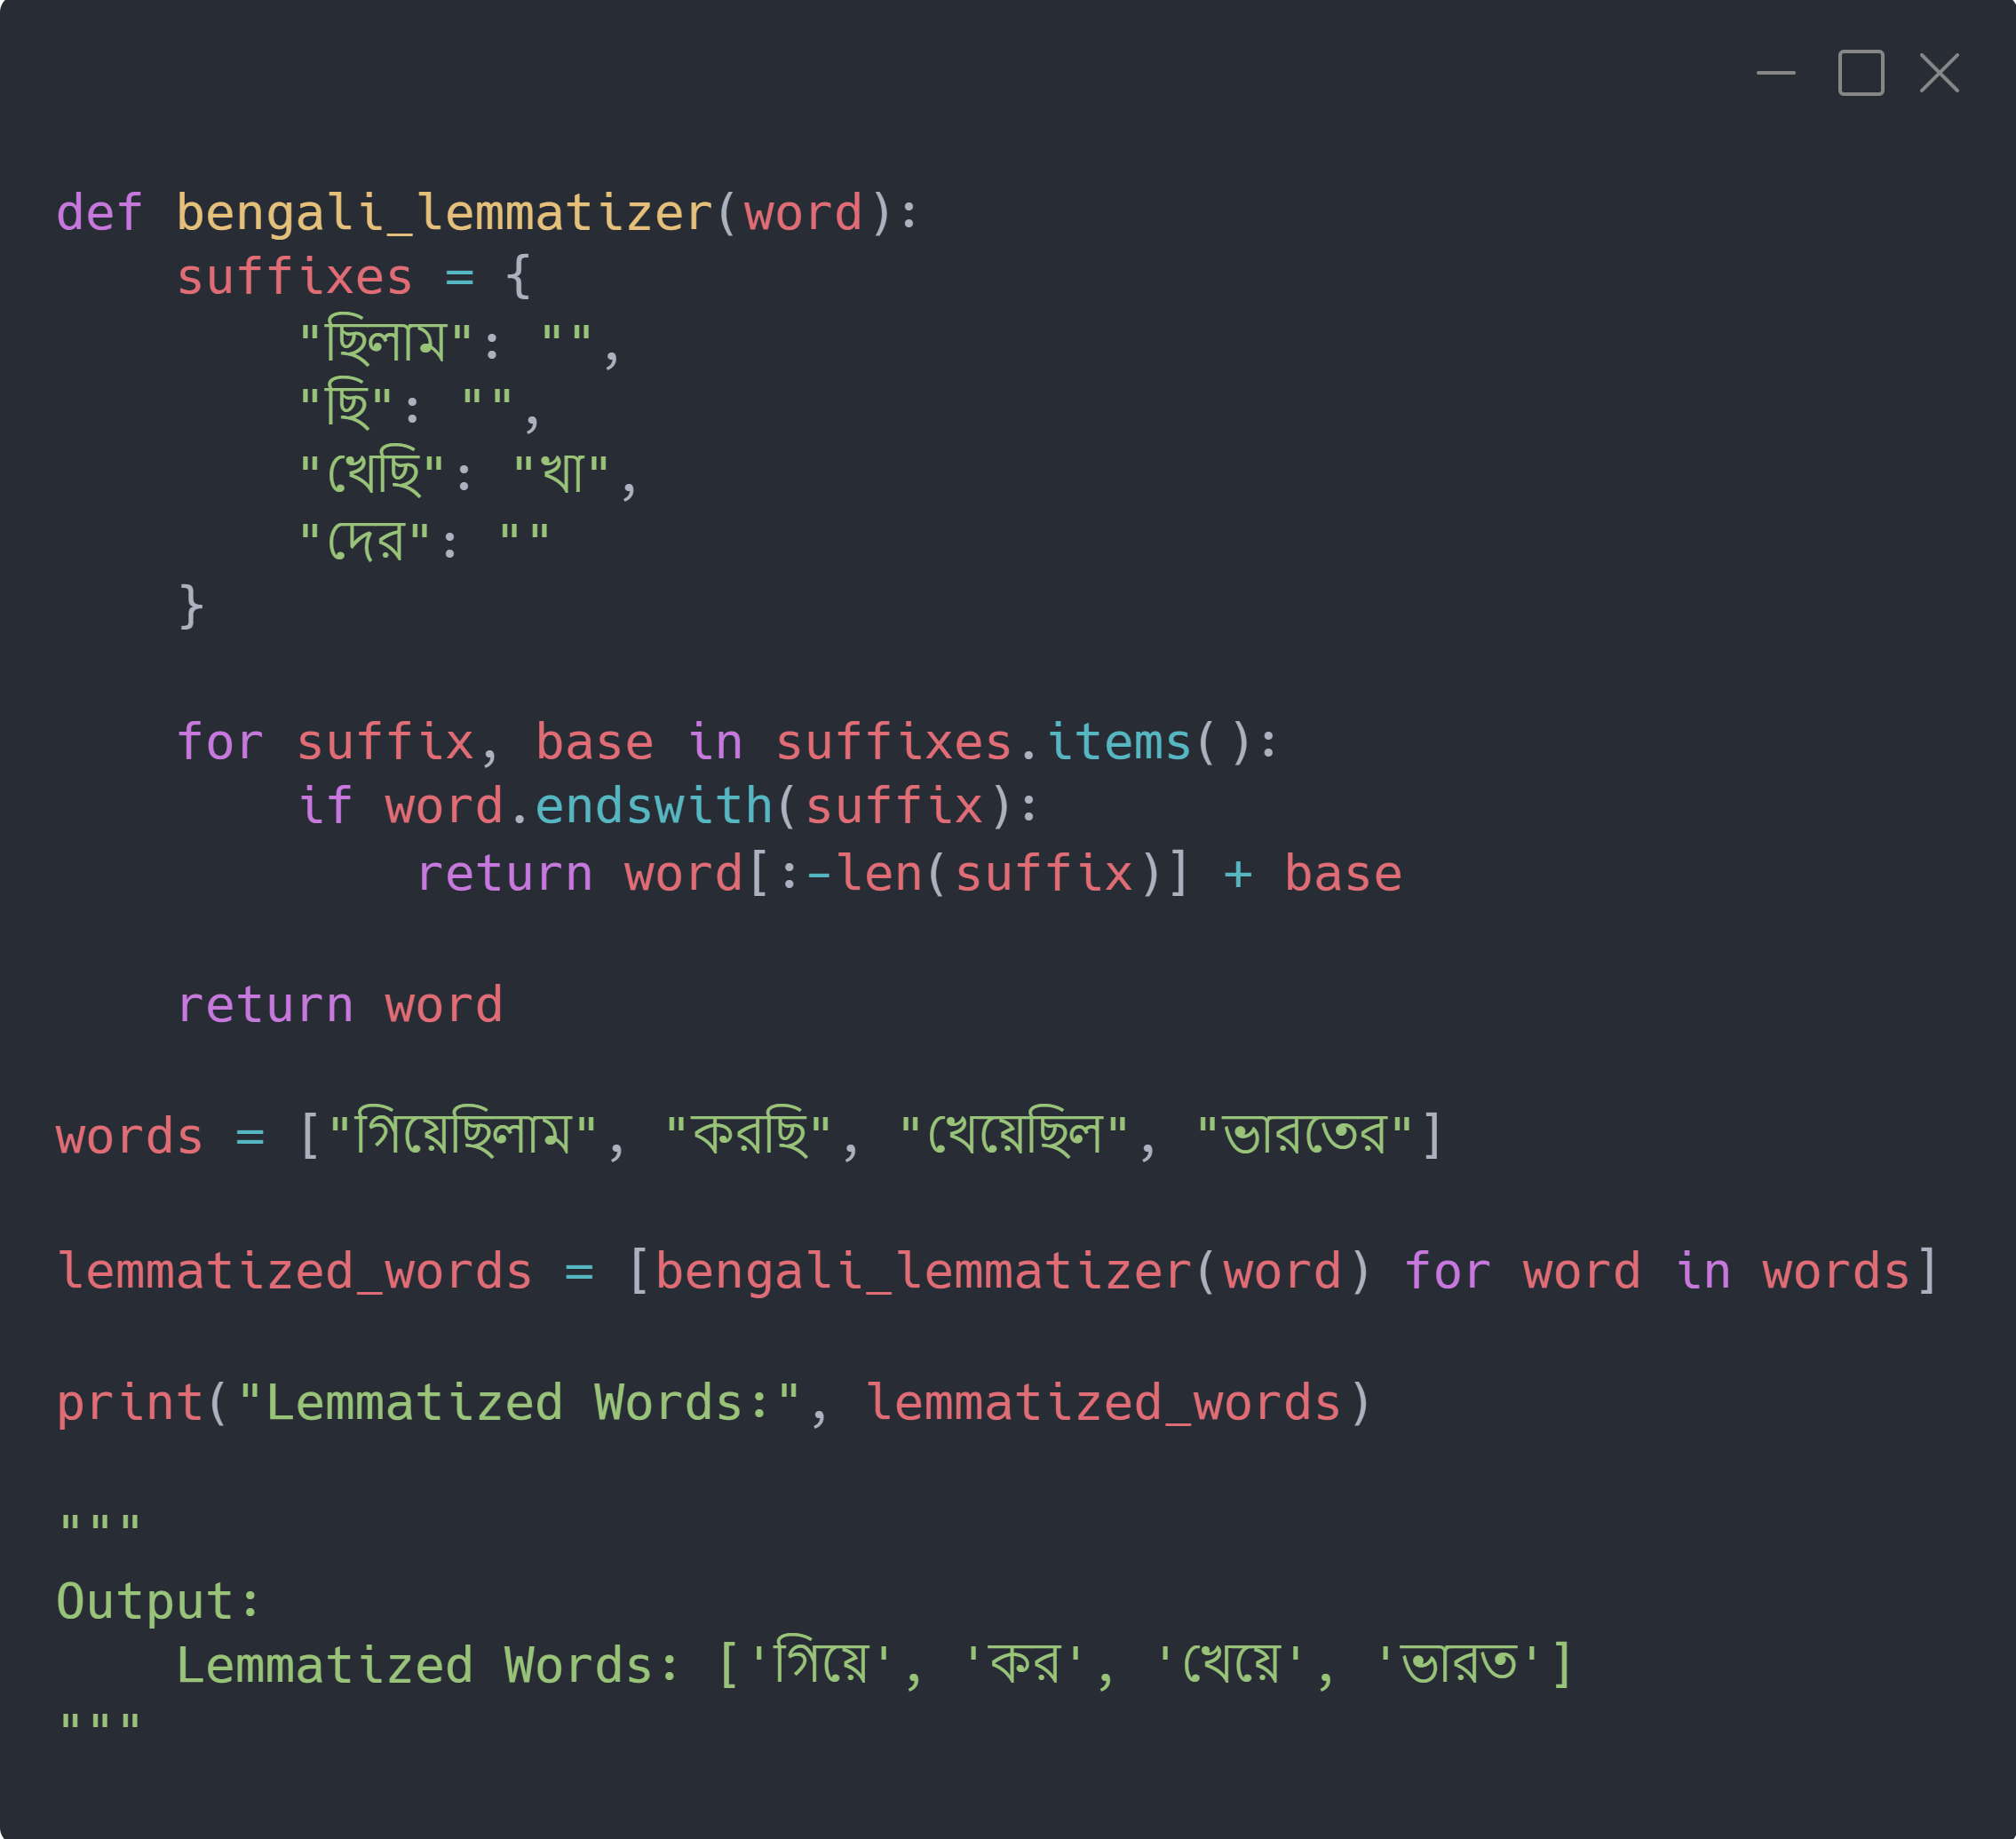
\includegraphics[width=0.8\linewidth]{Attachments/Figures/base-of-a-word_figure1.png}
    \caption{Illustration of Lemmatization in Bengali text.}
\end{figure}